\chapter{Felhasználói dokumentáció}

\section{A megoldott feladat}

A program lehetővé teszi a prímek néhány statisztikájának ábrázolását grafikonon,
és összevetését elméleti becsült értékekkel, valamint néhány különböző szita-algoritmus
futási idejének megmérését, és grafikus megjelenítését.
A programmal egyéb forrásból származó minták megjelenítése is lehetséges.

A prímszámok statisztikáinak előállításához a programhoz tartozik egy optimalizált
szita-implementáció, amivel $2^{64}$-ig lehet szitálni, és az eredményt rögzíteni.
Az elmentett prímlistákat a program egy külön része összesíti több statisztika szerint,
és a megjelenítést az összesítések alapján végzi el.

Különböző szita-algoritmusok futási idejének összehasonlításához a program tartalmazza
Atkin\cite{atkin} szitájának egy implementációját,
és Eratoszthenész szitájának néhány variációját.

\section{Felhasznált módszerek}

A program két elkülönülő részből áll. A prímszámok statisztikáinak
előállításához először szükséges a prímek listájának előállítása.
Ehhez egy optimalizált, gyors szita C nyelven készült el.
A könnyebb implementálhatóság miatt ez is két külön program, a kis
számokat szitáló init, és a nagyobb számokkal dolgozó generator.
A két program a működési elvében hasonló.

A program többi része Java nyelven van megírva, ez a gui nevű program.
Ez összesíti a prímek listáját, tartalmazza a futási idők összehasonlításához
írt szitákat, és jeleníti meg a prímek statisztikáit, és a futási idők
mintáit.

A program több prímszitát tartalmaz.
A prímsziták számok egy listájáról döntik el, hogy melyik szám prím, és melyik összetett.
A legtöbb implementált szita Eratoszthenész szitájának variációja.
Eratoszthenész szitája az egész számok egy adott $[2, n]$ intervallumába
eső számokról dönti el, hogy melyik prím.
Ezt a $pq$ szorzatra bontható számok megjelölésével teszi,
ahol a $p<n$ prím, és $1<q\in\mathbb{N}$.
Az algoritmus sorban veszi a számokat a listában kettőtől.
Ha egy addig még meg nem jelölt számot talál,
akkor az prím, és a listában megjelöli annak többszöröseit, de a prímet nem.
Az algoritmus futása után a meg nem jelölt számok a prímek.

\begin{algorithmic}[1]
\State n: \text{a szitálás felső határa}
\State \text{a számok legyenek nem megjelölve, 2-től $n$-ig}
\For{$i \gets 2$, $i \le n$, $i \gets i+1$}
	\If{$i$ nincs megjelölve}
		\For{$j \gets 2i$, $j \le n$, $j \gets j+i$}
			\State \text{legyen $j$ megjelölve}
		\EndFor
	\EndIf
\EndFor
\end{algorithmic}

Ennek az egyszerű algoritmusnak a legnagyobb hátránya,
hogy $n$-ig szitálva $n-1$ bit memóriára van szüksége,
ez a bitvektor a szitatábla.
Erre megoldás a szegmentált szitálás, ahol egy rövidebb,
nem feltétlenül 2-től kezdődő intervallumban szitálnak.
Ehhez szükség van a prímek listájára, legalább az intervallum végének négyzetgyökéig.

A legegyszerűbb szegmentált szita egy szegmens szitáláshoz
minden prímet sorban vesz, osztással meghatározza, hogy melyik a legkisebb
többszöröse a szegmensben, ha van ilyen szám,
majd onnantól összeadással szitál a szegmens végéig,
ahogy Eratoszthenész szitája is teszi.

Több, egymás utáni szegmens szitálásával az osztás
költsége több szegmensre szétosztható, ha a szita
a minden prímről minden szegmens szitálása után megjegyzi,
hogy melyik számot szitálna, ami már nagyobb, mint a szegmens vége.
A következő szegmens feldolgozásakor a prímmel innen lehet folytatni a szitálást.
A módszer hátránya, hogy ehhez el kell tárolni ezeket a prím-pozíció párokat,
ennek tárigénye nagyságrendileg $\mathcal{O}(\sqrt{n})$, ha legnagyobb
szitált szám $n$.
A hatékony eratoszthenészi sziták ennek a prím-pozíció listának
csak azon elemeit veszik figyelembe egy szegmens szitálásakor,
amik ténylegesen szitálnak is a szegmensben.

\subsection{Init és generator program}

A prímszámok listájának generátora C nyelven készült el.
A program csak parancssorból futtatható, és a sztenderd könyvtári függvényekből
is csak néhányat használ a memóriájában előállított eredmények fájlba írásához.
A C nyelv választását a hatékony végrehajtás és memóriafelhasználás, és
a hordozhatóság indokolja, a generátor elkülönítését az automatizálhatóság indokolja.

A prímgenerátor Eratoszthenész szitájának szegmentált változata,
a szitatábla egy $2^{30}$ hosszú darabját szitálja ki minden iterációban.
A generátor önmaga is két részből áll.
Egy egyszerűbb implementáció a prímek listáját $2^{32}$-ig állítja elő.
Ez az első 4 szegmens nem csak a statisztikákhoz szükséges,
a generator, és a Java program szitái is használja,
amikor a szitálás intervalluma 1-nél nagyobb számtól kezdődik.

A gyorsabb, de összetettebb szita $2^{32}$-től $2^{64}-2^{34}$-ig szitál,
és a futásához szükséges a prímek listája $2^{32}$-ig.
A szitatáblát a memóriában a gyorsítótár hatékonyabb a kihasználásához kisebb
részszegmensekre osztja,
és a prímeket a nagyságuk és a következő szitálási pozíciójuk szerint csoportosítja.
Továbbá nagyobb prímeknek csak harminccal relatív prím többszöröseit veszi figyelembe.

\subsection{Gui}

A program többi része a Java környezethez készült.

A program az adatbázisában hosszabb távon egyedül a prímek szegmensenkénti statisztikáit tárolja,
amit csak sorban dolgoz fel, és a statisztikák összmérete sem indokolna egy egyszerű bináris fájlnál bonyolultabb megoldást.
Az adatvesztés elkerüléséhez elég a statisztikafájl csere alapú felülírása.

A program a mintákat alapfüggvények lineáris kombinációjával közelíti a legkisebb négyzetek módszerével. A minták elemeinek nagy száma, és a mintaértékek
nagy terjedelme miatt szükséges volt a numerikus algoritmusok nagyobb pontosságú
implementációja, ami a számítási idő növekedésével jár.

A gui program tartalmaz több prímszita implementációt is, ezeknek az algoritmikus
bonyolultsága különböző, de a futási idejük összehasonlíthatóságához a közös részek közös
implementációt kaptak, és az eltérő részek hasonló szinten optimalizáltak.
A sziták helyességének ellenőrzéséhez a sziták eredménye egymással összehasonlítható.

A programhoz elkészült Eratoszthenész szitájának több variációja, mindegyik szegmentáltan működik,
a különbség a prímek listájának kezelésében van.
A legegyszerűbb implementált eratoszthenészi szita a prímek listáját minden szegmensben végig bejárja.
A prioritásos soron alapuló sziták a prímeket részlegesen rendezik az alapján, hogy hány szegmensnyire van az éppen szitált szegmenstől a prím következő többszöröse, a sor elejéről eltávolítják a szegmensben szitáló prímeket, és az új pozíciójukkal a sorba visszahelyezik.
Ilyen a bináris kupacot, és az edénysort használó szita.

A Cache Optimalizált Lineáris Szita a prímeket teljesen rendezi az alapján, hogy legközelebb melyik szegmensben fognak szitálni, és a prímek nagyság szerinti csoportosításával a rendezés fenntartásához az elemek memóriabeli mozgatását is kerüli.

Atkin szitája\cite{atkin} az előbbi algoritmusoktól jelentősen eltér, a prímek többszörösei
helyett $n=ax^2+by^2$ egyenlet megoldásait keresi egy $n$ szám vizsgálatához, $x$ és $y$ pozitív egészek befutásával, $a$ és $b$ egész konstansok.
A pontos kvadratikus formát, és $x$ és $y$ lehetséges értékeit Atkin az egészek algebrai bővítésével határozza meg, $n \in 4\mathbb{Z}+1$ esetén a Gauss-egészek, $n \in 6\mathbb{Z}+1$ esetén az Eisenstein-egészek, és $n \in 12\mathbb{Z}+11$ esetén a $\mathbb{Z}[\sqrt{3}]$ segítségével.

A sziták között kapott helyet a próbaosztás, és az erős pszeudoprím teszt\cite{pseudoprime} is, de ezek a lassúságuk miatt csak igen rövid tartományokon használhatóak.
A próbaosztás egy faktorizációs eljárás, ami egyetlen számot nem-triviális szorzatra próbál bontani.
Az (erős) pszeudoprím teszt egy prímteszt, egyetlen számról próbálja eldönteni, hogy az prím-e.
A prímteszteket általában több nagyságrenddel nagyobb számokra alkalmazzák, mint a szitákat, és teljes módszer helyett sokszor megelégednek egy valószínűségi válasszal.

\section{A program telepítése és futtatása}

A program futtatásához Windows vagy Linux operációs rendszer szükséges,
legalább 4GB szabad memóriával.
A Java program futtatásához JRE8 szükséges, a fordításához JDK8.
A C program fordításához C99 szabványú fordítóprogram kell.  A program fejlesztése és tesztelése OpenJDK8-cal és GCC 7.3-mal történt
Linux operációs rendszeren.

%%% EMIL: A másik dolog amit támogatok hogy beírod a github repo url-jét is.
A CD mellékleten található tarball a Java programot lefordítva is tartalmazza,
kicsomagolás után azonnal futtatható.
A C programot a generator könyvtárban található Makefile segítségével lehet lefordítani:
\begin{lstlisting}[language=bash]
generator$ make clean build
\end{lstlisting}

A Java program a NetBeans 8-as verziójával készült,
parancssorból a project ant fájlának segítségével lehet
újrafordítani:
\begin{lstlisting}[language=bash]
gui$ ant clean jar
\end{lstlisting}

A program futtatásához több előkészített script is rendelkezésre áll,
ezeket mind a scripts könyvtárból lehet indítani.
Az előző két fordítást egyben is el lehet végezni a recompile scripttel:
\begin{lstlisting}[language=bash]
scripts$ ./recompile
\end{lstlisting}

\section{Prímek keresése}

A prímek keresését két program végzi, az init program
$2^{32}$-ig keresi meg és tárolja el a prímeket,
a generator $2^{32}$-től $2^{64}-2^{43}$-ig.
Az init készítette szitattáblák a generator futásához szükségesek.

Mindkét program a számokat $2^{30}$ hosszú táblánkként szitálja,
minden tábla első száma $2^{30}k+1$ alakú.
A szitatáblában csak a páratlan számok vannak nyilvántartva.
A szitatáblákat a programok a
fájlrendszerben bitvektorként tárolják, egy tábla kb. $64$Mb.

Az első négymilliárd szám szitálása a következő képpen indítható el:

\begin{lstlisting}[language=bash]
generator$ ./init.bin ../db
szegmens 0 - kezdet             1 - felkészülés 159 906 063 ns - szitálás 1 122 878 403 ns
szegmens 1 - kezdet 1 073 741 825 - felkészülés   2 353 698 ns - szitálás 1 171 101 336 ns
szegmens 2 - kezdet 2 147 483 649 - felkészülés   2 344 515 ns - szitálás 1 188 330 478 ns
szegmens 3 - kezdet 3 221 225 473 - felkészülés   2 391 660 ns - szitálás 1 199 900 603 ns
\end{lstlisting}
Ennek eredmény 4 bittérképfájl, amit a db mappába ment.

A generator programot több féle képpen is lehet indítani.
Mindegyik esetben két paramétert kell megadni az indításhoz,
a számot, ahol szitálást kezdje, és a szegmensek számát, amit
ebben a futásban végig kell szitálni.
A kezdő számot meg lehet adni decimálisan is, vagy hexadecimálisan is,
"0x" prefixszel. A szegmensek számát is kétféle képpen lehet szabályozni.
Az egyik lehetőség fix számú szegmens megadása, decimálisan, vagy hexadecimálisan.

\begin{lstlisting}[language=bash]
generator$ ./generator.bin ../db start 0x100000001 segments 3
szegmens kezdet: 4 294 967 297
szegmensek száma: 3
kis szegmensek mérete: 22
elágazások bitjei: 8
felkészülés 1/4
felkészülés 2/4
felkészülés 3/4
felkészülés 4/4
felkészülés vége
szegmens 4 - kezdet 4 294 967 297 - felkészülés 8 162 031 487 ns - szitálás 729 914 370 ns
szegmens 5 - kezdet 5 368 709 121 - felkészülés           418 ns - szitálás 736 412 117 ns
szegmens 6 - kezdet 6 442 450 945 - felkészülés           385 ns - szitálás 750 022 409 ns
összes szitálás 2 216 348 896 ns
\end{lstlisting}

A másik mód a háttértáron fenntartandó szabad hely átadása, decimálisan,
vagy "0x" prefixszel hexadecimálisan. Ekkor következő szegmens szitálása előtt
megvizsgálja, hogy van-e még annyi szabad hely az adatbáziskönyvtárban, mint
amennyi meg van adva, ha igen, akkor szitálja a szegmenst,
és lép a következőre,
és ha nincs már elég szabad hely, akkor a program megáll.

\begin{lstlisting}[language=bash]
generator$ ./generator.bin ../db start 0x100000001 reserve-space 1000000000
szegmens kezdet: 4 294 967 297
fenntartandó hely: 1 000 000 000 byte 
kis szegmensek mérete: 22
elágazások bitjei: 8
felkészülés 1/4
felkészülés 2/4
felkészülés 3/4
felkészülés 4/4
felkészülés vége
szegmens 4 - kezdet 4 294 967 297 - felkészülés 8 162 031 487 ns - szitálás 729 914 370 ns
szegmens 5 - kezdet 5 368 709 121 - felkészülés           418 ns - szitálás 736 412 117 ns
szegmens 6 - kezdet 6 442 450 945 - felkészülés           385 ns - szitálás 750 022 409 ns
összes szitálás 2 216 348 896 ns
\end{lstlisting}

Mindkét program kimenetében a start a szegmens kezdőszáma, a segment az indexe,
$start=segment \cdot 2^{30}+1$, az init a szita inicializálási ideje a szitálás előtt,
és a sieve a szegmens szitálásának ideje. Ezek az információk az elmentett
táblafájlokból is kiolvashatóak.

\section{Mintaadatbázis karbantartása}

A mintaadatbázis a szitatáblák összesített statisztikáit tárolja.
A programok az adatbázis könyvtárában kétfajta fájlt vesznek figyelembe.
A szegmensek szitatáblái a {\tt''primes\textbackslash.[0-9a-f]\{16\}''} reguláris kifejezésnek megfelelő nevű fájlok.
A fájlnév második fele a szegmens kezdőszáma hexadecimálisan.
A fájl a páratlan számok bittérképe mellett tartalmazza a szegmens
szitálásának megkezdésére, és a szitálására fordított időt,
valamint ellenőrzésképpen a szegmens kezdőszámát is.

A szitatáblák mellett az adatbázis tartalmazhatja szegmensek összesített
statisztikáit is, ''aggregates'' néven. Ez a fájl az eddig összesített
szegmensekről a következő információkat tartja nyilván,
minden szegmensről külön-külön:
\begin{itemize}
\item a szegmens kezdőszáma
\item a szegmens szitálására való felkészülés idejét
\item a szegmens szitálásának idejét
\item az összesítésre fordított időt
\item a szegmensfájl utolsó módosítási idejét
\item a szegmensbe eső legkisebb, és legnagyobb prímet
\item a szegmensbe eső prímek számát,
$12\mathbb{Z}+11$, $4\mathbb{Z}+1$, $4\mathbb{Z}+3$, $6\mathbb{Z}+1$ alakok szerinti bontásban
\item a szegmensben előforduló prímhézagok első előfordulásának helyét,
és az előfordulások számát.
\end{itemize}

Példaként ha a szegmensek mérete 16 szám lenne,
és 17-től szitálnánk egy szegmens, akkor a szegmensfájl
leírná, hogy a prímek 17, 19, 23, 29, 31,
és az összetett számok 15, 21, 25, 27.
A szegmens összesítése
\begin{itemize}
\item a szegmens 17-tel kezdődik
\item a legkisebb prím 17, a legnagyobb 31
\item a szegmensben 5 darab prím van,
	ebből 2db $4\mathbb{Z}+1$,
	3db $4\mathbb{Z}+3$, 2db $6\mathbb{Z}+1$,
	és 1db $12\mathbb{Z}+11$ alakú
\item a szegmensben előforduló prímhézagok
\begin{itemize}
\item 2 (ikerprímek) kétszer fordul elő, először 17-nél
\item 4 egyszer fordul elő, először 19-nél
\item 6 egyszer fordul elő, először 23-nál
\end{itemize}
\end{itemize}
lenne.

Az adatbázison három művelet végezhető:
\begin{itemize}

\item Le lehet kérni, hogy
\begin{itemize}
\item a szegmensfájlok száma
\item az első és utolsó szegmensfájl
\item az legkisebb hiányzó szegmensfájl
\item a szegmensstatisztikák száma
\item az első és utolsó szegmensstatisztika
\item az legkisebb hiányzó szegmensstatisztika
\item van-e szegmensfájl, ami nincs összesítve
\end{itemize}

\item Összesíteni lehet az új szegmensfájlokat.

\item Össze lehet fésülni két összesítőfájlt.

\end{itemize}

Mindhárom művelet elvégezhető grafikus felületen, és automatizáláshoz parancssorból is.
A grafikus felületet a gui scripttel lehet indítani, a parancssorból
a database script segítségével lehet elérni a műveleteket.

Ezek a scriptek határozzák meg, hogy a program melyik könyvtárat használja
adatbázisként, ezt nem kell külön megadni.
Szükség esetén ez a könyvtár a scriptek egyszerű módosításával
megváltoztatható.

\subsection{Adatbázis információk}

A adatbázis információkat a grafikus felületen a ''DB info'' gomb megnyomásával lehet
lekérdezni, parancssorból a ''database info'' kiadásával.

\begin{lstlisting}[language=bash]
scripts$ ./database info
100.0%
szegmensfájlok: szegmensek száma: 7
szegmensfájlok: első szegmens kezdete: 1
szegmensfájlok: utolsó szegmens kezdete: 6,442,450,945
szegmensfájlok: első hiányzó szegmens kezdete: 7,516,192,769
szegmensfájlok: hiányzó szegmensek száma: 18,446,744,073,709,551,593

összesítések: szegmensek száma: 62,881
összesítések: első szegmens kezdete: 1
összesítések: utolsó szegmens kezdete: 67,516,885,893,121
összesítések: első hiányzó szegmens kezdete: 67,517,959,634,945
összesítések: hiányzó szegmensek száma: 18,446,744,073,709,488,719

új szegmensfájlok: 7

scripts$ ./database info crunch 1024
100.0%                     
szegmensfájlok: szegmensek száma: 4
szegmensfájlok: első szegmens kezdete: 1
szegmensfájlok: utolsó szegmens kezdete: 3,221,225,473
szegmensfájlok: első hiányzó szegmens kezdete: 4,294,967,297
szegmensfájlok: hiányzó szegmensek száma: 18,446,744,073,709,551,596

összesítések: szegmensek száma: 140,292
összesítések: első szegmens kezdete: 1
összesítések: utolsó szegmens kezdete: 150,636,314,230,785
összesítések: első hiányzó szegmens kezdete: 150,637,387,972,609
összesítések: hiányzó szegmensek száma: 18,446,744,073,709,411,308

crunch: ../generator/generator.bin /stuff/unistuff/scratch/szakdolgozat/db
start 0x890100000001 segments 0x400
\end{lstlisting}

A ''crunch'' utótag és szitálni kívánt szegmensek számának megadásával az utolsó sorban
a következő futtatásra ajánlott parancsot is megjeleníti a program.
Ezeknek a parancsoknak a követésével a teljes szitálható tartományt fel lehetne dolgozni.
A ''crunch-numbers'' script ezt a feladatot kísérli meg elvégezni.

Az info megjeleníti az új szegmensfájlok számát is, azokat,
amikhez vagy nem tartozik összesített adat, vagy tartozik,
de az ott tárolt utolsó módosításnál újabb a szegmensfájl.

\begin{figure}[h]
\centering
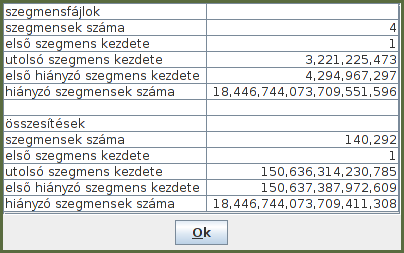
\includegraphics[scale=1]{info.png}
\end{figure}

\subsection{Szegmensek összesítése}

Az adatbázis könyvtárban
található új szegmensfájlokat a ''DB összesítés'' gomb megnyomásával,
vagy a ''database reaggregate'' paranccsal lehet összesíteni.
Minden olyan szegmensfájlról új összesítés készül,
amihez még nem tartozott összesítés, vagy a szegmensfájl
újabb, mint ami alapján a már meglévő összesítés készült.
Az adatbázisban már meglévő, többi szegmenshez tartozó statisztika nem vész el.

\begin{lstlisting}[language=bash]
scripts$ ./database reaggregate
100.0%
\end{lstlisting}

\subsection{Összesítőfájlok összefésülése}

Lehetőség van egy másik adatbázisból statisztikák átvételére is.
Erre több gépen párhuzamosan szitálva lehet szükség.
Az összefésülést a grafikus felületen a ''DB import'' megnyomása után
egy file kiválasztásával lehet indítani, parancssorból a ''dabatase import aggregates fájlnév''
kiadásával. A megadott fájlból azokat a szegmeneseket veszi át a program,
amik vagy nincsenek még meg az adatbázisban, vagy megvannak, de az importált
statisztikák utolsó módosítási ideje nagyobb az adatbázisban lévőnél.

\begin{lstlisting}[language=bash]
scripts$ ./database import aggregates ../db/aggregates.large
100.0%
\end{lstlisting}

%%% EMIL: ezt a részt kicst kuszának tartom. Én személy szerint, lehet úgy csinálnam, pl (feltéve hogy már rendesen bevezetted a generátor, init, stb programokat), és akkor először felsorolnám a műveleteket, hogy egy-egy program milyen parancsokat tud, aztán meg külön külön leírnám azok működését. Valahogy "nem elég száraz" a szöveg, egymásba folynak a mondatok... és szerintem itt most épp egy kicsit szárazabb, szakmaibb leírás kellene.

\section{Szitatáblák ellenőrzése}

A generator program teszteléséhez a grafikus program képes a szegmensfájlok ellenőrzésére.
Ehhez a program újra előállítja az ellenőrzött szegmensfájlokat, és azokat összeveti.
Az összevetéshez az egyszerű szegmentált eratoszthenészi szitát, vagy ez erős pszeudoprím tesztet lehet választani.
A pszeudoprím teszt rendkívül lassú, a célja, hogy a szitákhoz képest egy alapvetően más módszer is rendelkezésre álljon az ellenőrzéshez.

A grafikus felületen a "Szegmensfájlok ellenőrzése" gomb megnyomása után lehet kiválasztani a szitálni kívánt szegmenseket, és a referencia előállításának módszerét, majd az "Ellenőrzés" gombbal lehet megkezdeni a tényleges folyamatot.

Az ellenőrzést parancssorból is lehet futtatni a check-segments szkripttel.
A szkript első paraméterében a referencia módszerét várja, ami lehet "sieve", vagy "test", a paraméterek maradéka az ellenőrizendő szegmensek kezdőszáma kell legyen.
Ha egy kezdet sincs megadva, akkor a program az adatbázis könyvtárban található összes szegmensfájlt ellenőrzi.

\begin{lstlisting}[language=bash]
scripts$ ./check-segments sieve
100.0%: A szegmensek helyesek.             

scripts$ ./check-segments sieve 0x1 0xc0000001
100.0%: A szegmensek helyesek.             

scripts$ ./check-segments test 0x1
100.0%: A szegmensek helyesek.             

\end{lstlisting}

Ha a kezdőszám nagyobb, mint $1$, a szitával ellenőrzéshez szükséges,
hogy az init program által előállított négy darab szegmensfájlt tartalmazza
az adatbáziskönyvtár, mert a szita kezdőszámra pozícionálásához a prímszámokat
innen olvassa fel a program.

\section{Sziták ellenőrzése}

Az sebességek összehasonlításához írt sziták eredményét is lehet ellenőrizni,
az összehasonlításhoz itt is a szegmensek ellenőrzésénél használt
egyszerű szegmentált szita a referencia.

A program grafikus felületén a "Sziták ellenőrzése" lehetőséget
választva ki kell választani az ellenőrizendő szitát, és az ellenőrizni
kívánt intervallum kezdő és végző számát.
A folyamat az "Ellenőrzés" gomb megnyomásával indítható.

Parancssorból is ellenőrizhetőek a sziták a "check-sieve" scripttel.
A script 3 paramétere a szita neve, és az intervallum kezdő-, és végszáma.
Az ellenőrizhető sziták nevei:

\begin{itemize}
\item atkin: Atkin szitája\cite{atkin}
\item cols: Cache Optimalizált Lineáris Szita
\item eratosthenes-segmented: Eratoszthenész szitájának szegmentált változata
\item bin-heap és bin-heap-inplace: Eratoszthenész szitája bináris kupaccal,
	az bin-heap-inplace a kupac javítását helyben végzi
\item buckets, buckets-n, buckets-simple: Eratoszthenész szitája, edénysorral

	a buckets-simple nem szegmentált, a buckets, és a buckets-n szegmentált.
	a buckets-n -ben az n helyére 1-től 8-ig a számrendszer bitjeit lehet megadni,
	pl. buckets-3 8as számrendszerben számol
\item trial-division: próbaosztás
\end{itemize}

A ''Sziták'' fejezetben található ezeknek a szitáknak a részletesebb leírása.

A sziták nevei listázhatóak a list-sieves scripttel, a describe-sieves script rövid leírást
is ad.

\begin{lstlisting}[language=bash]
scripts$ ./check-sieve buckets-3 3000000000001 3010000000001
100.0%: A szita helyes.
\end{lstlisting}

Ha a kezdőszám nagyobb, mint egy, az ellenőrzéshez ilyenkor is szükséges,
hogy a négy darab kezdő szegmensfájlt tartalmazza az adatbáziskönyvtár.

\begin{figure}[h]
\centering
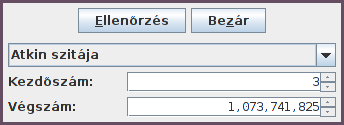
\includegraphics[scale=1]{check-sieve.png}
\end{figure}

\section{Minta megjelenítése}

A program a grafikus felületén képes mintákat ábrázolni, a mintákat függvényekkel
közelíteni, és ezeket a függvényeket is ábrázolni, valamint kiszámolja a közelítések
négyzetes hibáját a mintához képest.
A program egyváltozós, egyértékű mintákat kezel,
azok között is a természetes számokhoz valós számokat
rendelőket.
A minta akár külső forrásból is származhat.

A grafikonábrázoló részt a gui-graph scripttel lehet indítani,
vagy a gui scripttel, majd a "Grafikon" gomb megnyomásával.

Az ablak bal oldalán jelennek meg a betöltött minták és közelítő függvények
grafikonjai. Minta és függvény hozzáadása után a grafikon megjelenített részét
a program úgy választja meg, hogy minden minta összes pontja ebbe a nézetbe essen.
A nézet a grafikon feletti gombokkal, vagy egérrel mozgatható, nagyítható, vagy
kicsinyíthető.
Az ''Auto.nézet'' gombbal a nézet a minták teljes terjedelmére visszaállítható.

Az ablak jobb oldala a betöltött minták kezelésére szolgál.
A felső harmada az összes betöltött mintát mutatja.
Az ablak jobb oldalának alsó két harmadában az itt kiválasztott minta részletei
látszódnak.

\begin{figure}[h]
\centering
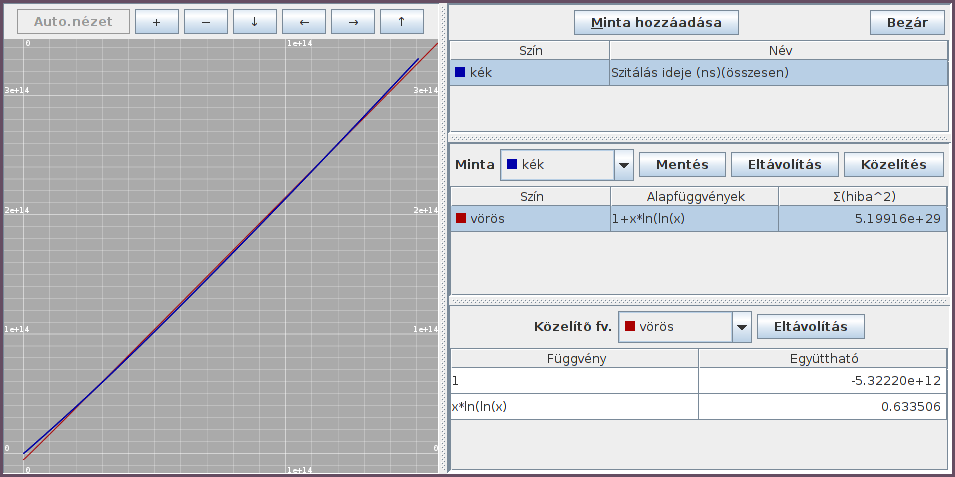
\includegraphics[scale=0.5]{graph.png}
\end{figure}

\subsection{Minta hozzáadása} %%% EMIL: Ez itt "hozzáadása" nem inkább beolvasása... betöltése... hmm... nem tom.

A "Minta hozzáadásánál" három adatforrásból lehet választani.
A "Fájl betöltésével" CSV fájl olvasható be. A fájl formátuma megengedő, az első oszlopot x, a második oszlopot y értékeknek próbálja értelmezni, a fel nem ismert sorokat eldobja.
Ha az első sor első oszlopa "BARS",
akkor vonaldiagram helyett a mintát oszlopdiagramként fogja ábrázolni.

A "Prímstatisztikák" a generator kimeneteléből összesített statisztikák, amiket az adatbáziskönyvtárban keres.
A program a szegmensstatisztikák hiánytalan kezdőszeletét veszi csak figyelembe.
A statisztikáknak három csoportja van. A prímek száma, és néhány kiemelt alakú prím száma a szegmensek végén. Ide tartozik ugyanezeken a helyeken a prímszámtétel becslése, és a becslés abszolút és relatív hibája is.
A prímhézagok statisztikái a szegmensek teljes kezdőszeletére vonatkozik.
Ezek az előfordult hézagok gyakorisága, első előfordulása, jósága, és az legnagyobb prímhézag adott számig.
Ezeken kívül a szegmensek szitálásának ideje is betölthető.
Az összesített idő a szegmensek végig az összes addigi szegmens összes ideje, a szegmensenkénti a szegmensek végéhez az adott szegmens szitálásának idejét rendeli.

A minták harmadik forrása a programba épített sziták futási idejének mérése.
Ehhez meg kell adni a szitát, a szitált intervallum elejét és végét, a szita belső szegmensméretét, a generálandó minták számát, és a mérések számát, a mértéket, és hogy az eredményt összesítse-e.
A sziták listája ugyanaz, mint a sziták ellenőrzősénél.
A mintákat a program a szitált intervallumon egyenletesen osztja el a megadott méretű szegmensek határainál.
A teljes szitálást a megadott mérések számászor végzi el, és az eredményt átlagolja.
Összesítést kiválasztva a minta értéke a szitált intervallum elejétől az adott számig szitálás teljes ideje, különben az előző minta helyétől.
A mérték szabályozza, hogy a tényleges eltelt időt mérje a program nanoszekundumban, vagy az elvégzett műveletek számát.

\subsection{Minta közelítése}

Az ablak jobb oldalának középső harmadában a kiválasztott minta részletei látszódnak.
Itt változtatható meg a minta ábrázolásához használt szín, távolítható el a minta,
vagy menthető CSV fájlba.

A táblázat a minta közelítéseit mutatja,
itt olvashatóak le a közelítés komponensfüggvényei, és a közelítés hibája.
A "Közelítés" gombbal lehet új közelítést hozzáadni az ábrázoláshoz.
A közelítéshez a lineáris legkisebb négyzetek módszerét használja a program,
ehhez a lineáris kombináció elemi függvényeit meg kell adni.
A függvények kiválaszthatóak az előre megadott listából,
vagy javascript nyelven is megadhatóak.
A közelítéshez csak olyan függvények használhatóak, amik a minta
minden pontjában értélmezve vannak.

Javascript függvényhez meg kell adni a függvény nevét és forráskódját.
A forráskódban a függvény argumentumára az $x$ változóval lehet hivatkozni,
és a script utolsó kifejezésének értéke lesz a függvény
értéke $x$-ben. Pl. az $x \mapsto \frac{\ln{x}}{x}$ hozzárendelés
forráskódja:

\begin{lstlisting}[basicstyle=\small, language=Java]
Math.log(x)/x
\end{lstlisting}

A scriptben használható változó, és a szokásos vezérlőutasítások.
Pl. az iterált logaritmus egy megadása:
\begin{lstlisting}[basicstyle=\small, language=Java,morekeywords=var]
var y=0;
while (1<x) {
  x=Math.log(x);
  ++y;
}
y
\end{lstlisting}

Az így megadott függvények visszatérési értéke mindig double kell legyen,
és a függvény azokban a pontokban értelmezett, ahol ez az érték véges.

Egy kiválasztott közelítés részletei az ablak jobb alsó sarkában látszódnak,
itt megváltoztatható a közelítéshez rendelt szín, és eltávolítható a közelítés.
A táblázat a közelítéshez kiválasztott függvények együtthatóit mutatja
a lineáris kombinációban.

A legkisebb négyzetek módszerének komponensei
röviden leírhatóak.
Ha az $n$ elemű minta
$(x_1, y_1), (x_2, y_2), ... (x_n, y_n)$
($x_i, y_i \in \mathbb{R}$),
a közelítéshez kiválasztott $m$ függvény
$f_1, f_2, ..., f_m$ ($f_i:\mathbb{R} \mapsto \mathbb{R}$),
akkor a legkisebb négyzetek módszere
keresi azokat a $c_1, c_2, ..., c_m$ ($c_i \in \mathbb{R}$)
skalárokat, hogy az
\begin{align*}
f(x)=\sum_{i=1}^m c_i f_i(x) (x \in \mathbb{R})
\end{align*}
közelítő függvény és a minta eltérése minimális
legyen a
\begin{align*}
\sum_{i=1}^{n} (f(x_i)-y_i)^2
\end{align*}
négyzetes eltérés összeg szerint.

A program ezt az eltérés összeget jeleníti meg a közelítés
hibájaként, valamint a $c_i$ skalárok
a közelítés elemi függvényeinek együtthatói.

\begin{figure}[h]
\centering
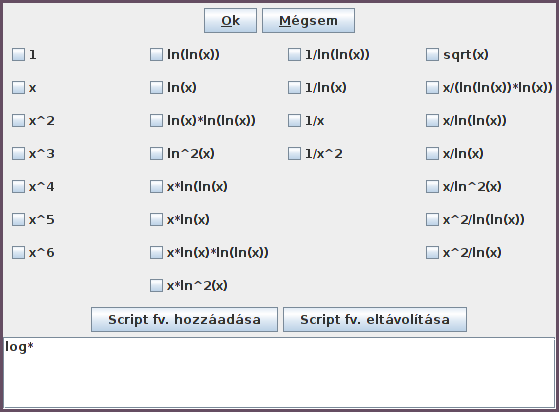
\includegraphics[scale=0.75]{functions}
\end{figure}

\section{Sziták mérése szkriptekkel}

%%% EMLI: Ez nem inkonzisztens? Eddi úgy volt hogy egy szekcióban egy funkció (csoportot) írtál le, és ott volt a GUI és CLI végrehajtás is, nem így külön szekcióban, nem? (és hogy a francba mondják magyarul a "sectiont"?)
A sziták futási idejének mintáit parancssorból is elő lehet állítani
a measure-sieve szkripttel, paraméterként meg kell adni ebben a sorrendben:

\begin{itemize}
\item a szita nevét, ezek ugyan azok lehetnek, mint a check-sieve szkriptnél
\item a számot, ahol a szitálás kezdődik, ez páratlan szám kell legyen
\item a szitálás végét, ez páratlan szám kell legyen
\item a szegmensek méretét
\item a mérések számát
\item a minták számát
\item hogy időt (nanosecs), vagy műveleteket (operations) mérjen
\item összesítse az időket (''sum''), vagy szegmensenként külön számolja (''segment'')
\item a fájlt, ahova az eredményt mentse CSV-ben
\end{itemize}

A számokat meg lehet adni decimálisan, és hexadecimálisan is "0x" előtaggal.
Ha a kezdőszám nagyobb, mint 1, akkor az adatbáziskönyvtárnak tartalmaznia
kell az init program generálta első négy szegmenst.

Lehetőség van a mérték és az összesítés mind a négy kombinációját egy
méréssel előállítani, ehhez mind a négy kimeneti fájl meg kell adni külön.

\begin{lstlisting}[language=bash]
scripts$ ./measure-sieve buckets-3 1 0x10000001 0x10000 3 1000 nanosecs sum out1.csv
100.0%
scripts$ ./measure-sieve buckets-3 1 0x10000001 0x10000 3 1000 operations segment out2.csv
100.0%
scripts$ ./measure-sieve buckets-3 1 0x10000001 0x10000 3 1000
seg-ns.csv seg-ops.csv sum-ns.csv sum-ops.csv
100.0%
\end{lstlisting}

A mérések megkönnyítéséhez a measure-sieves szkript az összes szitát megméri, és az eredményt a samples könyvtárba menti.
A samples könyvtárban a mérési eredmények 4 külön könyvtárban szegmensenként/összesítve, és idő/művelet szerinti bontásban vannak.
Ezekben a könyvtárakban 2 fajta mérés eredményei vannak.
Az atkin könyvtárban Atkin szitájának sebessége van megmérve különböző szegmensméretek esetén.
A speed kezdetű könyvtárakban az összes szita sebességének mérése található, $2^{20}$ szegmensmérettel.
A könyvtárak nevében a szám a szitálás kezdetét adja meg, a speed$n$ könyvtárban a mérések $2^n+1$-től kezdődnek.
A lassabb szitákat csak kisebb nagyságrendekre méri meg a szkript, ezek futási ideje hamar túl naggyá válik.

A measure-generator szkript a generator program sebességét méri meg, 3 változóban.
A szitálás kezdetének nagyságrendjén kívül a szegmensméretet, és az edénysor számrendszerét is variálja.
Az eredményt a samples/measure-generator.csv fájlba menti, ez nem használható a program mintamegjelenítésével, mert az egy változós mintákkal dolgozik.
Ennek a mérésnek a célja az, hogy a generator program paramétereit egy konkrét számítógéphez lehessen
igazítani.
A script 16 egymás utáni szegmensfájlt szitál, a szitálás kezdetét $2^{33}$-től $2^{63}$-ig változtatja, a kitevőt hármasával növelve, a szegmensek méretét $2^{16}$-tól $2^{24}$-ig, a kitevőt egyesével növelve, és a számrendszert $2^1$-től $2^8$-ig, szintén a kitevőt egyesével növelve.

%%% Local Variables:
%%% mode: latex
%%% TeX-master: "szakdolgozat"
%%% End:
